\documentclass[11pt, oneside]{article}  
\usepackage{amsmath, amssymb} % Math packages
\usepackage[margin=0.5in]{geometry} % Margins
\usepackage[ampersand]{easylist} % Bullets for lists
\usepackage{subcaption} % Side by side
\usepackage{csquotes} % Quotes
\usepackage{pgfplots} % Plotting
\usepackage{tikz} % Graphs
\usetikzlibrary{arrows.meta} % Arrows for nodes
\pgfplotsset{width=10cm,compat=1.9}
\usepackage[bottom]{footmisc}  %Glue footnotes to bottom
\usepackage{graphicx}
\graphicspath{ {imgs/} }

\title{Coursera-Stanford-ML-Notes}
\author{Quentin Truong}
\date{20 June 2017 - ? July 2017}


\begin{document}
\maketitle
\tableofcontents
\pagenumbering{arabic}
\clearpage



%======================================================
%========================WEEK 1========================
%======================================================
\section{Week 1: Introduction}
\subsection{Overview}
	\begin{easylist}  
	\ListProperties(Hide=100, Hang=true, Progressive=4ex, Style*=--\ , Style2*=$\bullet\ $)
		& Machine Learning: \hyphenquote{}{A computer program is said to learn from experience E with respect to some class of tasks T and performance measure P, if its performance at tasks in T, as measured by P, improves with experience E.}
		& Supervised Learning: know what our correct output looks like
		&& Regression: want continuous output
		&& Classification: want discrete output
		& Unsupervised Learning: little or no idea what our results should look like
		&& Clustering: find groups according to similarity in various variables 
		&& Nonclustering: find structure in chaos
	\end{easylist}

\clearpage



%======================================================
%========================WEEK 2========================
%======================================================
\section{Week 2: Linear Regression with Multiple Variables}
\subsection{Overview}
	\begin{easylist} 
	\ListProperties(Hide=100, Hang=true, Progressive=4ex, Style*=--\ , Style2*=$\bullet\ $)
		& Use linear regression for continuous output
		& Choose gradient descent if many features (million+) because the inverse matrix required for the normal equation can become expensive to compute
		& Normal equation will directly compute theta
		& Normalize features if using gradient descent
	\end{easylist}

\subsection{Notation}
	\begin{align*}
		m &= number\ of\ samples\\
		n &= number\ of\ feature\\
		x &= (n \times 1)\\
		X &= (m \times n)\\
		X_j &= (m \times 1)\\
		\theta &= (n \times 1)\\
		\theta_j &= (1 \times 1)
	\end{align*}

\subsection{Gradient Descent}
	\begin{align*}
		\text{Hypothesis Function} && 
			h_\theta(x) &= \theta^\intercal \times x\\
		\text{Vectorized Hypothesis Function} && 
			h_\theta(X) &= X \cdot \theta \\
		\text{Linear Regression Cost Function} && 
			J(\theta) &= \frac{1}{2 m} \sum (h_\theta(X) - y)^2 \\
		\text{Derivative of Linear Regression CF wrt $\theta_j$} && 
			\frac{\partial}{\partial \theta_j} J(\theta) &= \frac{1}{m} \sum (h_\theta(X) - y)\ .* X_j \\
		\text{Change in $\theta_j$} &&
			\theta_j &= \theta_j - \alpha \frac{\partial}{\partial \theta_j} \\
		\text{} &&
			&= \theta_j - \alpha \frac{1}{m} \sum (h_\theta(X) - y)\ .* X_j \\
		\text{Vectorized Change in $\theta$} &&
			\theta &= \theta - \alpha \frac{1}{m} X^\intercal (X \cdot \theta - y) 
	\end{align*}

\subsection{Normal Equation}
	\begin{align*}
		\theta &= (X^\intercal \cdot X)^\text{-1} \cdot X^\intercal \cdot y
	\end{align*}

\clearpage



%======================================================
%========================WEEK 3========================
%======================================================
\section{Week 3: Logistic Regression}
\subsection{Overview}
	\begin{easylist} 
	\ListProperties(Hide=100, Hang=true, Progressive=4ex, Style*=--\ , Style2*=$\bullet\ $)
		& Use logistic regression for discrete output (classification)
		&& $h_\theta(x)=(y=1|x;\theta)$; gives probability that the output is 1 given $x$
		&& Sigmoid/Logistic function maps any real number to (0, 1)
		&& Logarithm turns sum into product, allowing easier differentiation without altering search space
		& For multi-class classification, use one-vs-all
		&& Pick class i that maximizes $h^i_\theta(x)$
		& Overfitting is when learned hypothesis fits training data well but fails to generalize; underfitting is when doesn't fit training data
		& Address overfitting by reducing number of features, model selection, and regularization
		&& Regularization results in simpler hypothesis and less overfitting
		&& Extremely large $\lambda$ will result in underfitting and gradient descent will fail to converge
		&& Do not regularize $\lambda_0$
		& Use other prewritten optimization algorithims (conjugate gradient, BFGS, L-BFGS) because they are faster
	\end{easylist}

\subsection{Logistic Regression Hypothesis Function}
	\begin{align*}
		\text{Sigmoid/Logistic\ Function} && 
			g(z) &= \frac{1}{1+e^{-z}} \\
		\text{Hypothesis\ Function} && 
			h_\theta(x) &= g(\theta^\intercal x) \\
		\text{} && 
			&= \frac{1}{1+e^{-\theta^\intercal x}} 
	\end{align*}

\subsection{Logistic Regression Cost Function}
	\begin{align*}
		Cost(h_\theta(x), y) &= 
			\begin{cases} 
				-\log(h_\theta(x)) \text{ if y = 1 } \\
				-\log(1 - h_\theta(x)) \text{ if y = 0}
			\end{cases}\\
		&= -y\log(h_\theta(x)) - (1-y)\log(1 - h_\theta(x)) \\
		J(\theta) &= \frac{1}{m} \sum^m_{i=1}\text{Cost}(h_\theta(x^i),y^i) \\
		J(\theta) &= \frac{-1}{m} \sum^m_{i=1} \left[y^i\log(h_\theta(x^i)) + (1-y^i)\log(1 - h_\theta(x^i))\right] 
	\end{align*}
\iftrue
	\begin{figure}[!h]
		\begin{subfigure}{.5\textwidth}
			\centering
			\begin{tikzpicture}[scale=0.6]
				\begin{axis}[
					axis lines = left,
					xmin=0, xmax=1, ymin=0, ymax=1,
					xlabel = $h_\theta(x)$,
					ylabel = {$f(x)$},
				]
				\addplot [
					domain=0:1,
					samples=100, 
					color=red,
				]
				{-ln(x)/ln(10)};
				\end{axis}
			\end{tikzpicture}
			\caption{if y=1}
			\label{fig:sub1}
		\end{subfigure}%
		\begin{subfigure}{.5\textwidth}
			\centering
			\begin{tikzpicture}[scale=0.6]
				\begin{axis}[
					axis lines = left,
					xmin=0, xmax=1, ymin=0, ymax=1,
					xlabel = $h_\theta(x)$,
					ylabel = {$f(x)$},
				]
				\addplot [
					domain=0:1,
					samples=100, 
					color=red,
				]
				{-ln(1-x)/ln(10)};
				\end{axis}
			\end{tikzpicture}
			\caption{if y=0}
			\label{fig:sub2}
		\end{subfigure}
	\end{figure}
\fi

\subsection{Proof of Logistic Regression Cost Function Derivative}
	\begin{align*}
		J(\theta) &= \frac{-1}{m} \sum^m_{i=1} [y^i\log(h_\theta(x^i)) + (1-y^i)\log(1 - h_\theta(x^i))] \\
		\log(h_\theta(x^i)) &= \log(\frac{1}{1+e^{-\theta x^i}}) = -\log(1+e^{-\theta x^i})\\
		\log(1 - h_\theta(x^i)) &= \log(1-\frac{1}{1+e^{-\theta x^i}})=\log(e^{-\theta x^i})-\log(1+e^{-\theta x^i})=-\theta x^i-\log(1+e^{-\theta x^i})\\
		J(\theta) &= -\frac{1}{m}\sum_{i=1}^m \left[-y^i(\log(1+e^{-\theta x^i})) + (1-y^i)(-\theta x^i-\log(1+e^{-\theta x^i}))\right]\\
		&= -\frac{1}{m}\sum_{i=1}^m \left[y^i\theta x^i - \theta x^i - \log(1+e^{-\theta x^i})\right]\\
		&= -\frac{1}{m}\sum_{i=1}^m \left[y^i\theta x^i -\log(e^{\theta x^i}) - \log(1 + e^{-\theta x^i})\right]\\
		&=-\frac{1}{m}\sum_{i=1}^m \left[y^i\theta x^i - \log(1+e^{\theta x^i})\right]\\
		\frac{\partial}{\partial \theta_j}y^i\theta x^i &= y^i x^i_j\\
		\frac{\partial}{\partial \theta_j}\log(1+e^{\theta x^i}) &= \frac{x^i_je^{\theta x^i}}{1+e^{\theta x^i}}\\
		&= \frac{{x^i_j}}{{1+e^{-\theta x^i}}}\\
		&= x^i_jh_\theta(x^i)\\
		\frac{\partial}{\partial \theta_j}J(\theta) &= -\frac{1}{m}\sum_{i=1}^m \left[y^i x^i_j - x^i_jh_\theta(x^i)\right]\\
		\frac{\partial}{\partial \theta_j}J(\theta) &= \frac{1}{m}\sum_{i=1}^m \left[h_\theta(x^i) - y^i\right]x^i_j
	\end{align*}
	Credit\footnote{https://math.stackexchange.com/questions/477207/derivative-of-cost-function-for-logistic-regression}

\subsection{Regularization}
	\begin{align*}
		\text{Regularizing Term} &&
			& \lambda \sum_{j=1}^n \theta_j^2\\
		\text{Regularized Linear Regression CF} &&
			J(\theta) &= \frac{1}{2 m} \sum_{i=1}^m (h_\theta(x^i) - y^i)^2 + \lambda \sum_{j=1}^n \theta_j^2\\
		\text{Regularized Logistic Regression CF} &&
			J(\theta) &= \frac{-1}{m} \sum^m_{i=1} \left[y^i\log(h_\theta(x^i)) + (1-y^i)\log(1 - h_\theta(x^i))\right] + \frac{\lambda}{2m} \sum_{j=1}^n \theta_j^2\\
		\text{Regularized GD (Lin/Log Regression)} &&
			& \begin{cases} 
				\theta_0 = \theta_j - \alpha \left[\frac{1}{m}\sum_{i=1}^m (h_\theta(x^i) - y^i)x_0^i\right]\\
				\theta_j = \theta_j - \alpha \left[\frac{1}{m}\sum_{i=1}^m (h_\theta(x^i) - y^i)x_j^i + \frac{\lambda}{m}\theta_j\right] \text{(j=1,2,...,n)}
			\end{cases}\\
		\text{Regularized Normal Equation} &&
			\theta &= (X^\intercal X + \lambda 
			\begin{bmatrix} 
				0 & 0 & \cdots & 0 \\
  				0 & 1 & \cdots & 0 \\
				\vdots  & \vdots  & \ddots & \vdots  \\
				0 & 0 & \cdots & 1 
			\end{bmatrix}_{n+1,n+1}
			)^{-1} X^\intercal y
	\end{align*}

\clearpage



%======================================================
%========================WEEK 4========================
%======================================================
\section{Week 4: Artificial Neural Networks Representation}
\subsection{Overview}
	\begin{easylist} 
	\ListProperties(Hide=100, Hang=true, Progressive=4ex, Style*=--\ , Style2*=$\bullet\ $)
		& Neural networks allow for non-linear classification in situations with many features
		&& Necessary b/c 100 features at 3rd level polynomials generates 170k features, which quickly becomes intractable
		&& \hyphenquote{}{One learning algorithm} hypothesis; you can see with your tongue : brain learns using one algorithm, not thousands of different programs
		&& Can have multiple hidden layers
		&& Can have multiple outputs (one-vs-all for multi-class classification)
		&& If network has $s_j$ units in layer $j$ and $s_{j+1}$ units in layer $j+1$, then $\Theta^j$ will be of dimension $s_{j+1} \times s_j+1$
		&&& The +1 comes from the addition in $\Theta^{(j)}$ of the bias node, $x_0$ and $\Theta_0^{(j)}$
		& Forward Propogation is used to predict based on learned parameters
		& Bias node gives each node a trainable constant value
		&& Allows bias weight to shift the activation curve left/right
		&& Other weights affect steepness
		& Fun fact: For image recognition, particular order of pixels does not matter for ANN (but does for humans), you just need to keep the convention the same
	\end{easylist}

\subsection{Notation}
	\begin{easylist} 
	\ListProperties(Hide=100, Hang=true, Progressive=4ex, Style*=--\ , Style2*=$\bullet\ $)
		& $g(x)$: sigmoid function
		& $\Theta^{(j)}$: matrix of weights controlling function mapping from layer j to layer j+1; each layer gets own $\Theta^j$
		& $\Theta_{j,0}, ..., \Theta_{j,n}$ weights corresponding to the inputs $a_0, ..., a_n$ going into $z_j$
		& $w_{0,j}, ..., w_{n,j}$ weights corresponding to the inputs $a_0, ..., a_n$ going into $z_j$
		& $z_k^{(j)}$: encompasses parameters inside of g function
		& $a_i^{(j)}$: \hyphenquote{}{activation} of unit i in layer j
	\end{easylist}

\subsection{Equations}
	\begin{align*}
		z_k^{(j)} &= \Theta_{k,0}^{(j-1)}x_0 + \Theta_{k,1}^{(j-1)}x_1 + ... + \Theta_{k,n}^{(j-1)}x_n \\
		&= \Theta_{k,0}^{(j-1)}a_0^{(j-1)} + \Theta_{k,1}^{(j-1)}a_1^{(j-1)} + ... + \Theta_{k,n}^{(j-1)}a_n^{(j-1)} \\
		z^{(j)} &= \Theta^{(j-1)}a^{(j-1)} \\
		a^{(j)} &= g(z^{(j)})
	\end{align*}\newpage

\subsection{Sample Three Layer System}
	\begin{figure}[!h]
	    \centering
	    \begin{minipage}{.5\textwidth}
	    	\centering
	        \begin{equation*}
				\begin{bmatrix} 
					x_0 \\
					x_1 \\
					x_2 \\
					x_3 \\
				\end{bmatrix}
				\rightarrow
				\begin{bmatrix} 
					a_1^{(2)} \\
					a_2^{(2)} \\
					a_3^{(2)} \\
				\end{bmatrix}
				\rightarrow
				h_\Theta(x)
			\end{equation*}
			\begin{align*}
				a_1^{(2)} &= g(\Theta_{1,0}^{(1)} x_0 + \Theta_{1,1}^{(1)} x_1 + \Theta_{1,2}^{(1)} x_2 + \Theta_{1,3}^{(1)} x_3) \\
				a_2^{(2)} &= g(\Theta_{2,0}^{(1)} x_0 + \Theta_{2,1}^{(1)} x_1 + \Theta_{2,2}^{(1)} x_2 + \Theta_{2,3}^{(1)} x_3) \\
				a_3^{(2)} &= g(\Theta_{3,0}^{(1)} x_0 + \Theta_{3,1}^{(1)} x_1 + \Theta_{3,2}^{(1)} x_2 + \Theta_{3,3}^{(1)} x_3) \\
				h_\Theta(x) &= g(\Theta_{1,0}^{(2)} a_0^{(2)} + \Theta_{1,1}^{(2)} a_1^{(2)} + \Theta_{1,2}^{(2)} a_2^{(2)} + \Theta_{1,3}^{(2)} a_3^{(2)})\\
				&= g(z^3)\\
				&= a_1^{(3)}
			\end{align*}
	    \end{minipage}%
	    \begin{minipage}{0.5\textwidth}
	    	\centering
	    	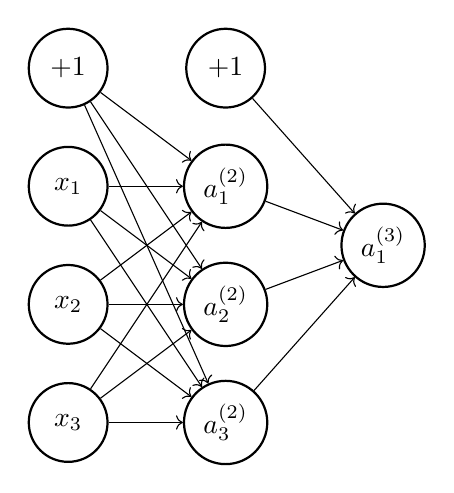
\begin{tikzpicture}
				\begin{scope}[every node/.style={circle,thick,draw,minimum size=10mm}]
					\node (x_0) at (0,4.5) {$+1$};
					\node (x_1) at (0,3) {$x_1$};
					\node (x_2) at (0,1.5) {$x_2$};
					\node (x_3) at (0,0) {$x_3$};

					\node (a_0^2) at (2,4.5) {$+1$};
					\node (a_1^2) at (2,3) {$a_1^{(2)}$};
					\node (a_2^2) at (2,1.5) {$a_2^{(2)}$};
					\node (a_3^2) at (2,0) {$a_3^{(2)}$};

					\node (a_1^3) at (4,2.25) {$a_1^{(3)}$};
				\end{scope}
				\begin{scope}[]
					\path [->] (x_0) edge node {} (a_1^2);
					\path [->] (x_0) edge node {} (a_2^2);
					\path [->] (x_0) edge node {} (a_3^2);

					\path [->] (x_1) edge node {} (a_1^2);
					\path [->] (x_1) edge node {} (a_2^2);
					\path [->] (x_1) edge node {} (a_3^2);

					\path [->] (x_2) edge node {} (a_1^2);
					\path [->] (x_2) edge node {} (a_2^2);
					\path [->] (x_2) edge node {} (a_3^2);

					\path [->] (x_3) edge node {} (a_1^2);
					\path [->] (x_3) edge node {} (a_2^2);
					\path [->] (x_3) edge node {} (a_3^2);

					\path [->] (a_0^2) edge node {} (a_1^3);
					\path [->] (a_1^2) edge node {} (a_1^3);
					\path [->] (a_2^2) edge node {} (a_1^3);
					\path [->] (a_3^2) edge node {} (a_1^3);
				\end{scope}
			\end{tikzpicture}
	    \end{minipage}
	\end{figure}

\clearpage



%======================================================
%========================WEEK 5========================
%======================================================
\section{Week 5: Artificial Neural Network Learning}
\subsection{Notation}
	\begin{easylist} 
	\ListProperties(Hide=100, Hang=true, Progressive=4ex, Style*=--\ , Style2*=$\bullet\ $)
		& $L$ : total number of layers in the network
		& $s_l$ : number of units (not counting bias unit) in layer $l$
		& $K$ : number of output units/classes
		& $h_\Theta(x)_k$ : hypothesis that results in the kth output
		& $\delta_k$ : Error signal 
	\end{easylist}

\subsection{Cost Function}
	\begin{equation*}
		J(\Theta) = - \frac{1}{m} \sum_{i=1}^m \sum_{k=1}^K \left[y^{(i)}_k \log ((h_\Theta (x^{(i)}))_k) + (1 - y^{(i)}_k)\log (1 - (h_\Theta(x^{(i)}))_k)\right] + \frac{\lambda}{2m}\sum_{l=1}^{L-1} \sum_{i=1}^{s_l} \sum_{j=1}^{s_{l+1}} ( \Theta_{j,i}^{(l)})^2
	\end{equation*}
	\begin{align*}
		\text{Picking training example} && 
			\sum_{i=1}^m\\
		\text{Picking output node} && 
			\sum_{k=1}^K\\
		\text{Picking layer} && 
			\sum_{l=1}^{L-1}\\
		\text{Picking node} && 
			\sum_{i=1}^{s_l}\\
		\text{Picking $\Theta$} && 
			\sum_{j=1}^{s_{l+1}}\\
	\end{align*}

\subsection{Backpropagation Algorithm}
	\begin{enumerate}
		\item Set $a(1):=x(t)$
		\item Perform forward propagation to compute $a(l)$ for $l=2,3,…,L$
		\item Using $y^{(t)}$, compute $\delta^L=a^{(L)} - y^{(t)}$
		\item Compute $\delta^{(L-1)}, \delta^{(L-2)},\dots,\delta^{(2)}$ using $\delta^{(l)} = ((\Theta^{(l)})^T \delta^{(l+1)})\ .*\ a^{(l)}\ .*\ (1 - a^{(l)})$
		\item $\Delta^{(l)}_{i,j} := \Delta^{(l)}_{i,j} + a_j^{(l)} \delta_i^{(l+1)}$ or with vectorization $\Delta^{(l)} := \Delta^{(l)} + \delta^{(l+1)}(a^{(l)})^\intercal$
		\item $\frac {\partial} {\partial \Theta_{ij}^{(l)}} J(\Theta) = D_{ij}^{(l)}$ where 
			$\begin{cases}
				D^{(l)}_{i,j} := \frac{1}{m}\Delta^{(l)}_{i,j} \text{ (j = 0)}\\
				D^{(l)}_{i,j} := \frac{1}{m}\left(\Delta^{(l)}_{i,j} + \lambda\Theta^{(l)}_{i,j}\right) \text{ (j $\neq$ 0)}\\
			\end{cases}$
	\end{enumerate}

\subsection{Backpropagation Derivation - Base Case}
	\begin{align*}
		\frac{\partial C}{\partial w_{ij}} &= \frac{\partial C}{\partial z_{j}} \frac{\partial z_{j}}{\partial w_{ij}} &&
			\text{Cost $C$ varies wrt input accumulator $z_j$, $z_j$ varies wrt $w_{ij}$ (Chain Rule)}\\
		\frac{\partial C}{\partial z_j} &= \frac{\partial}{\partial z_j} (y_j - a_j)^2 &&
			\text{Cost defined as $(y_j - a_j)^2$}\\
		&= \frac{\partial}{\partial z_j} (y_j - g(z_j))^2\\
		&= -2(y_j - g(z_j))g^\prime(z_j)\\
		g^\prime(z_j) &= \frac{d}{dz_j} \frac{1}{1+e^{-z_j}} &&
			\text{Derivative of logistic function}\\
		&= \frac{1}{1+e^{-z_j}} \frac{e^{-z_j}}{1+e^{-z_j}}\\
		&= g(z_j) (1-g(z_j))\\
		\frac{\partial C}{\partial z_j} &= -2(y_j - g(z_j))g(z_j)(1-g(z_j))\\
		&= -2(y_j - a_j)a_j(1-a_j)\\
		\frac{\partial z_{j}}{\partial w_{ij}} &= \frac{\partial}{\partial w_{ij}} \sum_q a_q w_{q,j} &&
			\text{Definition of $z_j$ as sum of previous node's inputs and their weights}\\
		&= a_i\\
		\frac{\partial C}{\partial w_{ij}} &= -2(y_j - a_j)a_j(1-a_j)(a_i)\\
		&= -\Delta_j a_i
	\end{align*}

\subsection{Backpropagation Derivation - Recursive Case}
	\begin{align*}
		\frac {\partial C}{\partial w_{i,j}} &= \sum_k (\frac{\partial C}{\partial z_k} \frac{\partial z_k}{\partial a_j} \frac{\partial a_j}{\partial z_j} \frac{\partial z_j}{\partial w_{i,j}})
			&& \text{$C$ depends on $z_k$, $z_k$ depends on $a_j$, $a_j$ depends on $z_j$, $z_j$ depends on $w_{i.j}$} \\
		\frac {\partial C}{\partial z_k} &= -\Delta_k\\
		\frac {\partial z_k}{\partial a_j} &= \frac {\partial}{\partial a_j} \sum_s a_s w_{s,k}\\
		&= w_{j,k}\\
		\frac {\partial a_j}{\partial z_j} &= \frac {\partial}{\partial z_j} g(z_j)\\
		&= g(z_j)(1-g(z_j))\\
		&= a_j(1 - a_j)\\
		\frac {\partial z_j}{\partial w_{i,j}} &= \frac {\partial}{\partial w_{i,j}} \sum_q a_q w_{q,j}\\
		&= a_i\\
		\frac {\partial C}{\partial w_{i,j}} &= \sum_k (-\Delta_k w_{j,k} a_j(1 - a_j) a_i)\\
		&= \sum_k (-\Delta_k w_{j,k}) a_j(1 - a_j) a_i\\
		&= -\Delta_j a_i
	\end{align*}
	Credit
	\footnote{https://pdfs.semanticscholar.org/69c2/814c7f8ca16aa836fd32e3c4975f8208e63f.pdf}
	\footnote{https://stats.stackexchange.com/questions/94387/how-to-derive-errors-in-neural-network-with-the-backpropagation-algorithm}
	\footnote{https://theclevermachine.wordpress.com/2014/09/06/derivation-error-backpropagation-gradient-descent-for-neural-networks/}

\subsection{Backpropagation Intuition}
	$\delta_k$ is the error signal from the output
	\begin{equation*}
		\delta_k = (a_k - t_k)g^\prime_k(z_k)
	\end{equation*}
	so, error wrt output weights is
	\begin{equation*}
		\frac {\partial E}{\partial w_{j,k}} = \delta_k a_j
	\end{equation*}
	similarly, error wrt internal weights is
	\begin{equation*}
		\frac {\partial E}{\partial w_{i,j}} = \delta_j a_i
	\end{equation*}
	the error is determined by following layer's error, so it may also be understood as
	\begin{equation*}
		\frac {\partial E}{\partial w_{i,j}} = g^\prime_j(z_j) \sum_k (\delta_k w_{j,k}) a_i
	\end{equation*}

\subsection{Gradient Checking}
\begin{easylist} 
	\ListProperties(Hide=100, Hang=true, Progressive=4ex, Style*=--\ , Style2*=$\bullet\ $)
		& Gradient checking ensures that backpropagation is actually working
		&& Turn off gradient checking once backpropagation is verified to work
		& Approximate the derivative of cost function using slope
		&& Pick $\epsilon = 10^{-4}$
		&& Check all $\Theta_j$
	\end{easylist}
	\begin{equation*}
		\dfrac{\partial}{\partial\Theta_j}J(\Theta) \approx \dfrac{J(\Theta_1, \dots, \Theta_j + \epsilon, \dots, \Theta_n) - J(\Theta_1, \dots, \Theta_j - \epsilon, \dots, \Theta_n)}{2\epsilon}
	\end{equation*}

\subsection{Random Initialization}
	\begin{easylist} 
	\ListProperties(Hide=100, Hang=true, Progressive=4ex, Style*=--\ , Style2*=$\bullet\ $)
		& Need Symmetry Breaking
		&& All hidden units would receive the same signal and the same updates
		&& Results in finding only one feature, redundantly copied many times over
		& Fixed by randomly initializing each $\Theta_{ij}^{(l)}$ to a value in $[-\epsilon, \epsilon]$
		&& A good choice of $\epsilon$ init is $\epsilon = \frac {\sqrt 6}{\sqrt{L_{in} + L_{out}}}$, where $L_{in} = s_l$ and $L_{out} = s_{l+1}$, the number of units in the layers adjacent to $\Theta^{(l)}$
	\end{easylist}

\clearpage



%======================================================
%========================WEEK 6========================
%======================================================
\section{Week 6: Advice for Machine Learning}
\subsection{Overview}
	\begin{easylist} 
	\ListProperties(Hide=100, Hang=true, Progressive=4ex, Style*=--\ , Style2*=$\bullet\ $)
		& Training set: 60\%
		& Cross validation set: 20\%
		& Test set: 20\%
		& Randomize your data and plot learning curves to determine high/low variance
	\end{easylist} 

\subsection{Evauating Hypothesis}
	\begin{align*}
		\text{Linear regression} && 
			J_{test}(\Theta) &= \dfrac{1}{2m_{test}} \sum_{i=1}^{m_{test}}(h_\Theta(x^{(i)}_{test}) - y^{(i)}_{test})^2\\
		\text{Classification} &&
			err(h_\Theta(x),y) &= 
				\begin{cases} 
					1 \text{ if } h_\Theta(x) \geq 0.5 \text{ and } y = 0\\
					1 \text{ if } h_\Theta(x) < 0.5 \text{ and } y = 1\\
					0 \text{ otherwise}
				\end{cases}\\
		\text{Test Error} &&
			&= \dfrac{1}{m_{test}} \sum^{m_{test}}_{i=1} err(h_\Theta(x^{(i)}_{test}), y^{(i)}_{test})
	\end{align*}
	
\subsection{Bias, Variance, Learning Curves}	
	\begin{easylist} 
	\ListProperties(Hide=100, Hang=true, Progressive=4ex, Style*=--\ , Style2*=$\bullet\ $)
		& High variance is when overfitting data
		&& Get more training examples, try a smaller set of features, increase lambda
		& High bias is when underfitting data
		&& Add features, add polynomial features, decrease lambda
		& Small neural networks are more prone to underfitting and are cheaper
		& Large neural networks are more prone to overfitting and are more expensive
	\end{easylist} 
	\begin{figure}[!h]
	\centering
	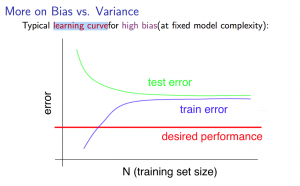
\includegraphics[scale=0.8]{learning_curve_HB}
	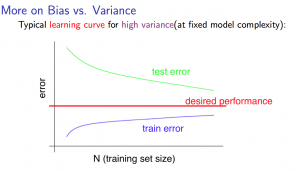
\includegraphics[scale=0.8]{learning_curve_HV}
	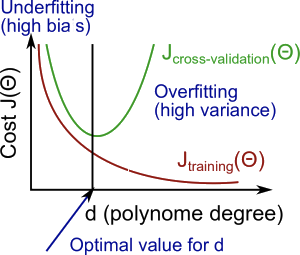
\includegraphics[scale=0.6]{learning_curve_D}
	\end{figure}

\clearpage



%======================================================
%========================WEEK 7========================
%======================================================
\section{Week 7: }





\end{document}  